\section{Controllo della molteplicit\al (family-wise error)}
\label{mtp}
\subsection{Why multiple testing?}

\begin{frame}{Many tests in one experiment}
  \bb{Genomics}
    One test for every gene or probe
  \eb
  \bb{Clinical trials}
    Multiple outcome measures or subgroups
  \eb
  \bb{Regression modeling}
    One t-test per regression coefficient
  \eb
  \bb{Anova}
    All pairwise comparisons in an anova model
  \eb
\end{frame}


\begin{frame}{Example: microarray study}
  \bb{Top 5 genes out of 20,000}
    {\scriptsize\begin{tabular}{lrr}
    Gene & p-value  \\ \hline
  OCIAD2 &5.5e-6  \\
    NEK3 &6.7e-6  \\
    TAF5 &7.1e-6  \\
 FOXD4L6 &7.5e-6  \\
    ADIG &8.8e-6  \\
  \textbf{\vdots} & \textbf{\vdots} \\\hline
  \end{tabular}}
  \eb
  \bb{Small p-value?}
    \bi
      \item Getting a p-value as small as 5.5e-6 is unlikely
      \item But is it also small if we admit that we tried 20,000 times?
      \item Can we reliably state that OCIAD2 is differentially expressed?
      \item What about NEK3?
    \ei
  \eb
\end{frame}

\begin{frame}{Probability of a false rejection}
  \bb{$K$ independent true hypotheses}
    Reject hypotheses if p-value smaller than $\alpha$
  \eb
  \bb{Probability of making a false rejection}
    $p = 1- (1-\alpha)^K$
  \eb
\end{frame}

\begin{frame}{Type I error if not correcting for multiple testing}%
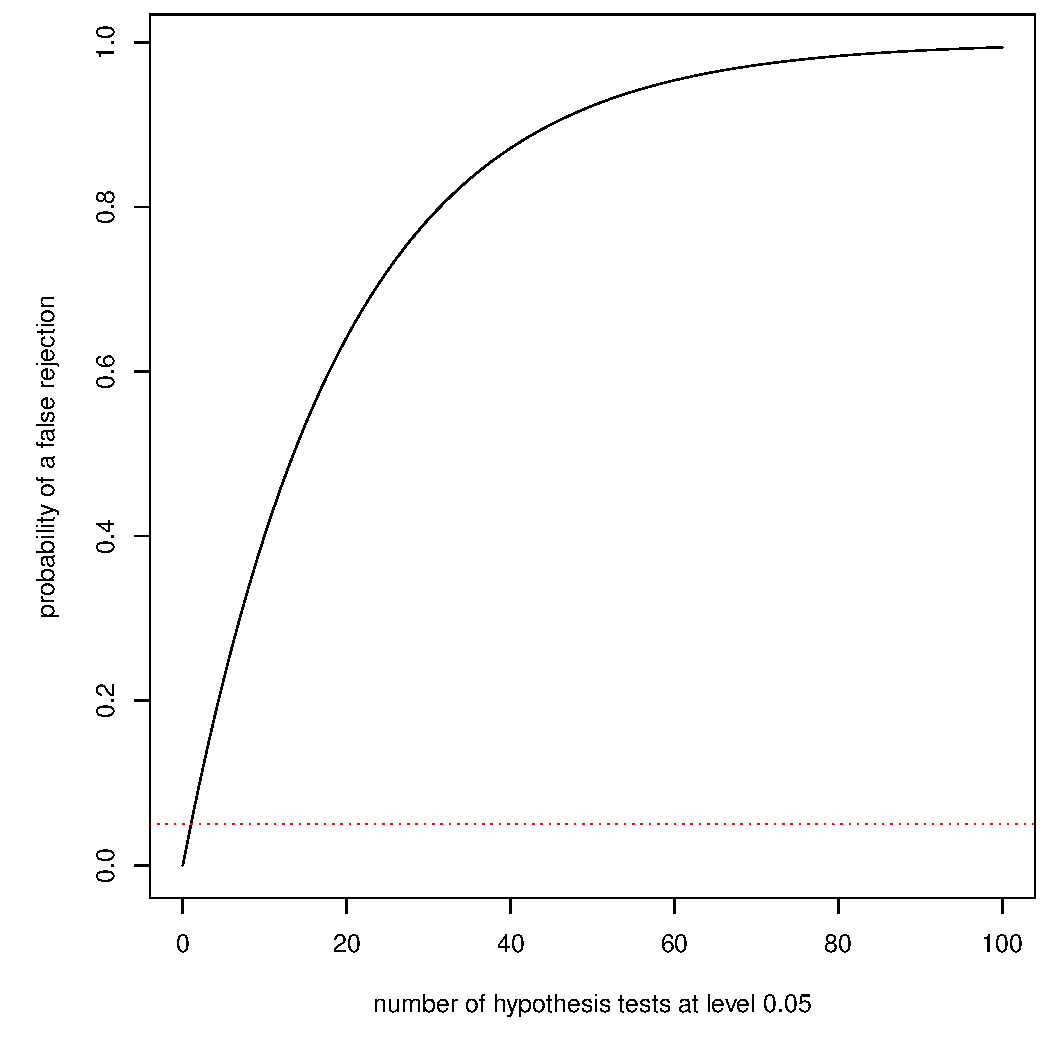
\includegraphics[height=7cm]{MTP/typeI}
\end{frame}


\begin{frame}{Type I errors}
  \bb{Single hypothesis $H_0$: type I error}
    Probability of rejecting $H_0$ when $H_0$ true $\leq \alpha$
  \eb
  \bb{This lecture}
    \bi
      \item How to define type I error with multiple hypotheses?
      \item How to protect against type I error?
    \ei
  \eb
\end{frame}



\subsection{Null hypotheses}

\begin{frame}{Hypotheses as subspaces of the parameter space}
\centering
\begin{tikzpicture}[scale=1]
\draw[help lines, <->] (-3.5,0)--(3.5,0);
\draw[help lines, <->] (0,-3.5)--(0,3.5);
\path (3.5,0) node[below left] {$\theta_1$};
\path (0,3.5) node[below right] {$\theta_2$};
\path (0,0) node[anchor=north west] {0};
\draw<2-> [red, very thick, <->] (0,-3.5,0)--(0,3.5);
\path<2-> [red] (3,3) node {$H_1: \theta_1=0$};
\draw<3-> [green, <->, very thick] (-3.5,0)--(3.5,0);
\path<3-> [green] (3,2) node {$H_2: \theta_2=0$};
\draw<4-> [blue, very thick, fill] (0,0) circle (1pt);
\path<4-> [blue] (3,1) node {$H_1 \cap H_2: \theta_1=\theta_2=0$};
\end{tikzpicture}
\end{frame}


\begin{frame}{True and false hypotheses}
  \bb{Hypotheses}
    $H_1,\ldots,H_m$
  \eb
  \bb{True hypotheses}
    A true hypothesis is a hypothesis that contains the true value of the parameter
  \eb
  \bb{Collection of true hypotheses}
    $T \subseteq \{1,\ldots,m\}$ indices of true hypotheses (unknown)
  \eb
\end{frame}



\begin{frame}{Familywise error rate}
  \bb{Rejections}
    $R \subseteq \{1,\ldots,m\}$ index set of rejected hypotheses
    \\ Typically a random variable
  \eb
  \bb{False rejections}
    Rejected true hypotheses $T \cap R$ (random)
  \eb
  \bb{Familywise error rate (FWER)}
    Probability of making a false rejection = $\mathrm{P}(T \cap R \neq \emptyset)$
  \eb
  \bb{Generalizes type I error}
    FWER = type I error if only one hypothesis is tested
  \eb
\end{frame}



\subsection{Boole}

\begin{frame}{Reminder: events}
  \bb{Outcome space}
    $\Omega$: collection of all possible outcomes of the experiment
  \eb
  \bb{Event}
    A subspace of $\Omega$
  \eb
  \centering
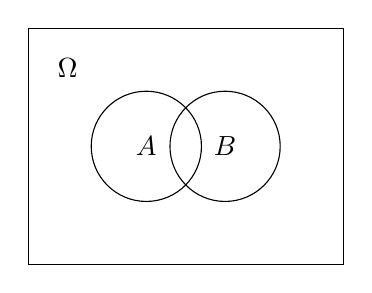
\begin{tikzpicture}
  \draw (0,0) rectangle (4,3);
  \draw (1.5,1.5) circle (.7 cm);
  \draw (2.5,1.5) circle (.7 cm);
  \path (1.5,1.5) node {$A$};
  \path (2.5,1.5) node {$B$};
  \path (.5,2.5) node {$\Omega$};
\end{tikzpicture}
\end{frame}

\begin{frame}{Boole}
  \bb{Boole's inequality}
    For any events $A$ and $B$:
    \[ \mathrm{P}(A \cup B) = \mathrm{P}(A) + \mathrm{P}(B) - \mathrm{P}(A \cap B) \]
    so
    \[ \mathrm{P}(A \cup B) \leq \mathrm{P}(A) + \mathrm{P}(B) \]
    For any events $A_1, \ldots, A_m$:
    \[ \mathrm{P}(\bigcup_{i=1}^m A_i) \leq \sum_{i=1}^m \mathrm{P}(A_i) \]
  \eb
  \bb{Equality}
    Equality holds if events are disjoint
  \eb
\end{frame}


\begin{frame}{P-values}
  \bb{Start from p-values}
    Often p-value $p_1,\ldots,p_m$ for each hypothesis available
  \eb
  \bb{Marginal property}
    P-values are uniformly distributed under the null hypothesis:\\
    $\mathrm{P}(p_i \leq \alpha) = \alpha$ if $H_i$ true (sometimes $\leq \alpha$)
  \eb
  \bb{Joint distribution}
    Joint distribution of p-values (dependence) often unknown
  \eb
\end{frame}


\section{Bonferroni, Holm and Shaffer}
\subsection{Single step (Bonferroni)}

\begin{frame}{The Bonferroni inequality}
  \bb{Reduced $\alpha$}
    Bonferroni: reduce significance level for each hypothesis
    \\ Reject $H_i$ if $p_i \leq \alpha/m$
  \eb
  \bb{Control of FWER}
    \begin{eqnarray*}
    \mathrm{FWER} &=& \mathrm{P} \big(\textrm{$p_i \leq \alpha/m$ for at least one $i$ with $H_i$ true} \big) \\
    &=& \mathrm{P} \Big( \bigcup_{i\in T} \{p_i \leq \alpha/m\} \Big) \\
    &\leq& \sum_{i \in T} \mathrm{P} (p_i \leq \alpha/m) \\
    &\leq& \#T\frac{\alpha}{m} \leq \alpha
    \end{eqnarray*}
  \eb
\end{frame}


\begin{frame}{Using Bonferroni}
  \bb{Advantages}
    \bi
      \item Extremely easy
      \item Strong control of FWER under any dependence of p-values
    \ei
  \eb
  \bb{Disadvantage}
    Conservative: FWER $\leq \alpha$, often $<\alpha$
  \eb
  \bb{When is Bonferroni least conservative?}
    \bi
      \item Events $\{p_i \leq \alpha/m\}$ disjoint
      \item $\# T = m$: complete null hypothesis
    \ei
  \eb
\end{frame}


\begin{frame}{Adjusted p-values}
  \bb{Bonferroni}
    Critical value $\alpha/m$ depends on number of hypotheses $m$
  \eb
  \bb{Alternative: ``multiplicity adjusted p-value''}
    Make $\tilde p_i = mp_i$ and compare with $\alpha$
  \eb
  \bb{General}
    Multiplicity-adjusted p-value is the smallest FWER $\alpha$ at which the hypothesis would be rejected in a multiple testing procedure
  \eb
  \bb{Compare}
    The definition of the regular p-value
  \eb
\end{frame}


\subsection{Sequential (Holm)}

\begin{frame}{Holm's procedure}
  \bb{Sequential Bonferroni}
    Start with $c = \alpha/m$
    \\ Repeat
    \be
      \item Reject all hypotheses with p-value $\leq c$
      \item Recalculate $c = \alpha/(m-r)$ \\ with $r$ number of so far rejected hypothesis
    \ee
  \eb
  \bb{Compare to Bonferroni}
    Larger critical values $\to$ less conservative
  \eb
\end{frame}


\begin{frame}{Holm: example}
  \bb{Example: p-values}
  \hspace*{-1cm}
  {\footnotesize
  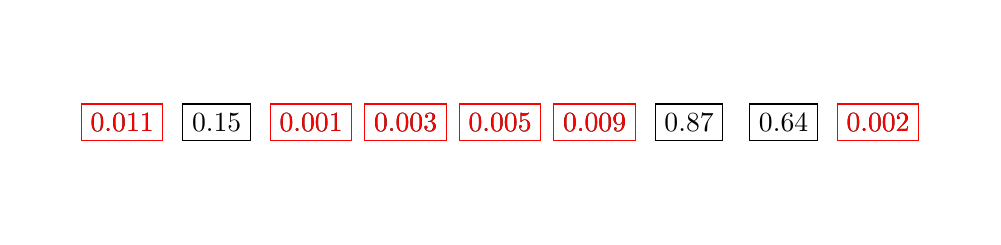
\begin{tikzpicture}[scale=1.2]
    \path (0,0) rectangle (10,2);
    \path (1,1) node[draw] {0.011};
    \path<6-> [red] (1,1) node[draw] {0.011};
    \path (2,1) node[draw] {0.15};
    \path (3,1) node[draw] {0.001};
    \path<2-> [red] (3,1) node[draw] {0.001};
    \path (4,1) node[draw] {0.003};
    \path<2-> [red] (4,1) node[draw] {0.003};
    \path (5,1) node[draw] {0.005};
    \path<2-> [red] (5,1) node[draw] {0.005};
    \path (6,1) node[draw] {0.009};
    \path<4-> [red] (6,1) node[draw] {0.009};
    \path (7,1) node[draw] {0.87};
    \path (8,1) node[draw] {0.64};
    \path (9,1) node[draw] {0.002};
    \path<2-> [red] (9,1) node[draw] {0.002};
  \end{tikzpicture}}
  \eb
  \bb{Critical value}
    \be
      \item 9 hypotheses, $\alpha=0.05$, so $c = 0.05/9 = 0.0056$
      \item<3-> 5 remaining hypotheses, $\alpha=0.05$, so $c = 0.05/5 = 0.01$
      \item<5-> 4 remaining hypotheses, $\alpha=0.05$, so $c = 0.05/4 = 0.0125$
      \item<7> 3 remaining hypotheses, $\alpha=0.05$, so $c = 0.05/3 = 0.0167$
    \ee
  \eb
\end{frame}


\begin{frame}{Holm's procedure controls FWER}
  \bb{Proof via critical event}
    \bi
      \item Define event $E$: all true hypotheses have p-value $> \alpha/(\#T)$
      \item $\mathrm{P}(E)\geq1-\alpha$ (compare proof of Bonferroni)
      \item If $E$ happens, no true hypothesis is rejected
      \item Consequence:
      \[
      \textrm{FWER} = \mathrm{P}(\textrm{at least one false rejection}) \leq 1-\mathrm{P}(E)\leq\alpha
      \]
    \ei
  \eb
  \bb{Compare to Bonferroni}
    Method is valid under the same general assumptions as Bonferroni
  \eb
\end{frame}


\subsection{Restricted combinations (Shaffer)}

\begin{frame}{Related hypotheses}
  \bb{Example}
    Anova model. Three subgroups.\\
    Hypotheses: pairwise comparisons between subgroups.
    \begin{eqnarray*}
      H_{12}&:& \mu_1=\mu_2\\
      H_{23}&:& \mu_2=\mu_3\\
      H_{13}&:& \mu_1=\mu_3
    \end{eqnarray*}
  \eb
  \bb{Relationships}
    If $H_{12}$ is false, $H_{23}$ and $H_{13}$ cannot be both true.
  \eb
  \bb{Restricted combinations}
    Not all combinations of truth/falsehood of hypotheses are viable
  \eb
\end{frame}


\begin{frame}{Shaffer's method}
  \bb{Variant of Holm's method with restricted combinations}
    Start with $c = \alpha/m$
    \\ Repeat
    \be
      \item Reject all hypotheses with p-value $\leq c$
      \item Recalculate $c = \alpha/s$ \\ with $s$ the maximum number of hypotheses that can still be true given that all the rejections made so far are correct
    \ee
  \eb
  \bb{Compare to Holm}
    Method is valid under the same general assumptions as Holm
    \\ Less conservative than Holm in case of restricted combinations
  \eb
\end{frame}

\begin{frame}{Shaffer: example}
  \bb{Hypotheses and data}
    \begin{eqnarray*}
      H_{12}&:& \mu_1=\mu_2 \qquad p_{12} = 0.01\\
      H_{23}&:& \mu_2=\mu_3 \qquad p_{23} = 0.04\\
      H_{13}&:& \mu_1=\mu_3 \qquad p_{13} = 0.53
    \end{eqnarray*}
  \eb
  \bb{Shaffer's procedure}
    \be
      \item Reject all hypotheses with p-value $\leq \alpha/3$ $\to$ reject $H_{12}$
      \item If $H_{12}$ is false, at most one of $H_{23}$ and $H_{13}$ can be simultaneously true
      \item Reject all hypotheses with p-value $\leq \alpha/1$  $\to$ reject $H_{23}$
      \item Continue:\ldots No further rejections possible
    \ee
  \eb
\end{frame}

